%==============================================================================
\section{DeltaSort Algorithm}
\label{sec:algorithm}
%==============================================================================

\subsection{Overview}

Before we get to how the algorithm works, let's establish useful terminology-

\begin{definition}[Direction]
\label{def:direction}
For an updated index $i$, we define its \emph{direction} based on local order:
\begin{itemize}
  \item \textbf{LEFT ($L$)}: Value \textbf{must} move left---$\texttt{cmp}(A[i-1], A[i]) > 0$ (for $i > 0$).
  \item \textbf{RIGHT ($R$)}: Value \textbf{may} move right and \textbf{cannot} move left.
\end{itemize}
\end{definition}

\begin{remark}
The definition of direction is deliberately asymmetric: L requires a definite violation ($A[i-1] > A[i]$), while R encompasses both violations and non-violations. One might consider a three-way classification with a separate S (stable) category for values already in their correct positions. However, this complicates the setup:
\begin{enumerate}
  \item S values need to be processed identically to R values (both may stay or move right).
  \item Fixing an R value can shift values, potentially converting a previously S neighbor into an R violation. Example: consider array $[20, 30, 10]$ where indexes $0$ and $1$ were updated. Index $0 (20)$ is initially S because it is correctly places w.r.t index $1$ $(30)$, but once index $1$ is fixed, index $0$ becomes an R violation since $20 > 10$. 
\end{enumerate}
The two-way classification avoids this issue by maintaining a useful invariant: \emph{the direction of an updated index never changes until it is repairedd}. This simplifies the implementation.
\end{remark}

\begin{definition}[Segment]
\label{def:segment}
A \emph{segment} is a pair of indices $(i, j)$ with $i < j$ satisfying:
\begin{enumerate}
  \item Either $i = 0$, or $i \in U$ with direction R.
  \item Either $j = n - 1$, or $j \in U$ with direction L.
  \item There do not exist updated indices $p, q \in U$ with $i < p < q < j$ such that $p$ has direction L and $q$ has direction R.
  \item There do not exist updated indices $p < $i and $q > $j such that $(p, q)$ is also a segment.
\end{enumerate}

More intuitively, a segment is a contiguous portion of the array where all R-direction updates precede all L-direction updates. Condition~(3) ensures that no L appears before an R within the segment. Condition~(4) ensures segments are maximal and non-overlapping. Conditions~(1) and~(2) handle boundary cases: a leading segment containing only L's is bounded by the array start, and a trailing segment containing only R's is bounded by the array end. \figref{fig:segment-structure} illustrates this structure.
\end{definition}

% Figure: Segment structure diagram
\begin{figure}[H]
\centering
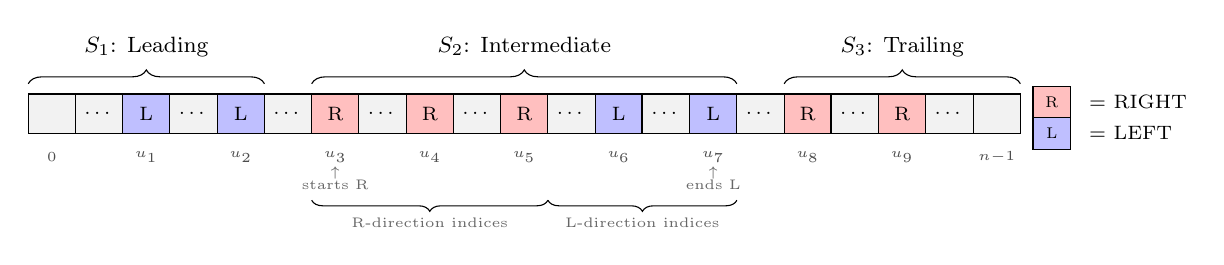
\begin{tikzpicture}[
    cell/.style={minimum width=0.6cm, minimum height=0.5cm, draw, font=\scriptsize},
    dotcell/.style={minimum width=0.5cm, minimum height=0.5cm, font=\scriptsize},
    indexcell/.style={minimum width=0.6cm, font=\tiny, text=black!70},
    right/.style={cell, fill=red!25},
    left/.style={cell, fill=blue!25},
    clean/.style={cell, fill=gray!10, font=\scriptsize},
    segbrace/.style={decorate, decoration={brace, amplitude=5pt}},
    segbracem/.style={decorate, decoration={brace, amplitude=4pt, mirror}},
    seglabel/.style={font=\footnotesize},
    condlabel/.style={font=\tiny, text=black!60},
    faded/.style={opacity=0.4}
]

% Array indices (shown below)
\def\yidx{-0.55}
\def\yarr{0}

% === ARRAY START ===
\node[clean] at (-0.9, \yarr) {};
\node[indexcell] at (-0.9, \yidx) {$0$};
\node[clean] at (-0.3, \yarr) {\dots};

% === LEADING SEGMENT (L's only, bounded by array start) ===
\node[left] (l0) at (0.3, \yarr) {L};
\node[indexcell] at (0.3, \yidx) {$u_1$};
\node[clean] at (0.9, \yarr) {\dots};
\node[left] (l1) at (1.5, \yarr) {L};
\node[indexcell] at (1.5, \yidx) {$u_2$};

% Inter-segment clean region
\node[clean] at (2.1, \yarr) {\dots};

% === MIDDLE SEGMENT (R's then L's) ===
\node[right] (r1) at (2.7, \yarr) {R};
\node[indexcell] at (2.7, \yidx) {$u_3$};
\node[clean] at (3.3, \yarr) {\dots};
\node[right] (r2) at (3.9, \yarr) {R};
\node[indexcell] at (3.9, \yidx) {$u_4$};
\node[clean] at (4.5, \yarr) {\dots};
\node[right] (r3) at (5.1, \yarr) {R};
\node[indexcell] at (5.1, \yidx) {$u_5$};
\node[clean] at (5.7, \yarr) {\dots};
\node[left] (l2) at (6.3, \yarr) {L};
\node[indexcell] at (6.3, \yidx) {$u_6$};
\node[clean] at (6.9, \yarr) {\dots};
\node[left] (l3) at (7.5, \yarr) {L};
\node[indexcell] at (7.5, \yidx) {$u_7$};

% Inter-segment clean region
\node[clean] at (8.1, \yarr) {\dots};

% === TRAILING SEGMENT (R's only, bounded by array end) ===
\node[right] (r4) at (8.7, \yarr) {R};
\node[indexcell] at (8.7, \yidx) {$u_8$};
\node[clean] at (9.3, \yarr) {\dots};
\node[right] (r5) at (9.9, \yarr) {R};
\node[indexcell] at (9.9, \yidx) {$u_9$};

% === ARRAY END ===
\node[clean] at (10.5, \yarr) {\dots};
\node[clean] at (11.1, \yarr) {};
\node[indexcell] at (11.1, \yidx) {$n{-}1$};

% === SEGMENT BRACES (top) ===
% Leading segment
\draw[segbrace] (-1.2, 0.38) -- (1.8, 0.38);
\node[seglabel] at (0.3, 0.85) {$S_1$: Leading};

% Middle segment
\draw[segbrace] (2.4, 0.38) -- (7.8, 0.38);
\node[seglabel] at (5.1, 0.85) {$S_2$: Intermediate};

% Trailing segment
\draw[segbrace] (8.4, 0.38) -- (11.4, 0.38);
\node[seglabel] at (9.9, 0.85) {$S_3$: Trailing};

% === SUB-BRACES for middle segment (bottom) ===
\draw[segbracem] (2.4, -1.1) -- (5.4, -1.1);
\node[condlabel, anchor=north] at (3.9, -1.2) {R-direction indices};
\draw[segbracem] (5.4, -1.1) -- (7.8, -1.1);
\node[condlabel, anchor=north] at (6.6, -1.2) {L-direction indices};

% === ANNOTATIONS for boundary conditions ===
% Condition markers (centered on cells)
\node[condlabel] at (2.7, -0.75) {$\uparrow$};
\node[condlabel] at (2.7, -0.9) {starts R};

\node[condlabel] at (7.5, -0.75) {$\uparrow$};
\node[condlabel] at (7.5, -0.9) {ends L};

% === LEGEND ===
\node[right, scale=0.8] at (11.8, 0.15) {R};
\node[font=\scriptsize, anchor=west] at (12.15, 0.15) {= RIGHT};
\node[left, scale=0.8] at (11.8, -0.25) {L};
\node[font=\scriptsize, anchor=west] at (12.15, -0.25) {= LEFT};

\end{tikzpicture}
\caption{A segment $(i,j)$ starts at either index $0$ or an R-direction updated index, and ends at either index $n{-}1$ or an L-direction updated index, with all R's preceding all L's within. In this example, the leading segment $S_1$ contains only L's (starting from index $0$), the intermediate segment $S_2$ contains R's followed by L's, and the trailing segment $S_3$ contains only R's (ending at index $n{-}1$). Leading and trailing segments may or may not be present depending on the directions of updated indices.}
\label{fig:segment-structure}
\end{figure}

Armed with these definitions, we can see how DeltaSort works. It operates in two phases:

\begin{enumerate}
  \item \textbf{Phase 1 (Segment):} Extract updated values, sort them, and write back to updated indices in index order. This establishes segments (\defref{def:segment}) in the array that are disjoint and can be \emph{repaired independently}.
  \item \textbf{Phase 2 (Repair):} Repair each segment left-to-right, deferring R indices to a stack until the first L index is encountered. When a L is encountered, first flush and repair all pending Rs in LIFO order, then repair the L. Continue left-to-right.
\end{enumerate}

\figref{fig:delta-sort-example} illustrates the full DeltaSort process on a small example.

% Example figure showing segmentation with concrete array
\begin{figure}[t]
\centering
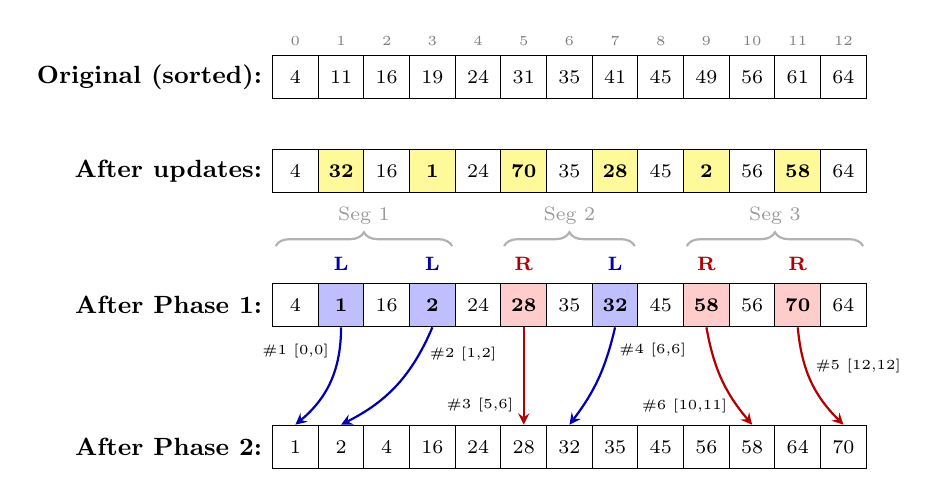
\begin{tikzpicture}[
    cell/.style={draw, minimum width=0.58cm, minimum height=0.55cm, font=\scriptsize},
    cellup/.style={cell, fill=yellow!40, font=\scriptsize\bfseries},
    cellL/.style={cell, fill=blue!25, font=\scriptsize\bfseries},
    cellR/.style={cell, fill=red!20, font=\scriptsize\bfseries},
    larrow/.style={->, >=stealth, thick, blue!70!black},
    rarrow/.style={->, >=stealth, thick, red!70!black},
    segbrace/.style={decorate, decoration={brace, amplitude=5pt}},
]

% === STAGE 1: Original sorted array ===
\node[font=\small\bfseries, anchor=east] at (-0.3, 0) {Original (sorted):};
\foreach \i/\v in {0/4, 1/11, 2/16, 3/19, 4/24, 5/31, 6/35, 7/41, 8/45, 9/49, 10/56, 11/61, 12/64} {
    \node[cell] (o\i) at (\i*0.58, 0) {\v};
}
% Index labels
\foreach \i in {0,...,12} {
    \node[font=\tiny, gray] at (\i*0.58, 0.45) {\i};
}

% === STAGE 2: After updates applied ===
\node[font=\small\bfseries, anchor=east] at (-0.3, -1.2) {After updates:};
\foreach \i/\v/\up in {0/4/0, 1/32/1, 2/16/0, 3/1/1, 4/24/0, 5/70/1, 6/35/0, 7/28/1, 8/45/0, 9/2/1, 10/56/0, 11/58/1, 12/64/0} {
    \ifnum\up=1
        \node[cellup] (u\i) at (\i*0.58, -1.2) {\v};
    \else
        \node[cell] (u\i) at (\i*0.58, -1.2) {\v};
    \fi
}

% === STAGE 3: After Phase 1 (sorted updates, L/R classified) ===
\node[font=\small\bfseries, anchor=east] at (-0.3, -2.9) {After Phase 1:};

% Segment braces (between Stage 2 and L/R labels)
\draw[segbrace, thick, gray!60] (0*0.58-0.25, -2.15) -- (3*0.58+0.25, -2.15) 
    node[midway, above=4pt, font=\scriptsize, gray!80] {Seg 1};
\draw[segbrace, thick, gray!60] (5*0.58-0.25, -2.15) -- (7*0.58+0.25, -2.15) 
    node[midway, above=4pt, font=\scriptsize, gray!80] {Seg 2};
\draw[segbrace, thick, gray!60] (9*0.58-0.25, -2.15) -- (12*0.58+0.25, -2.15) 
    node[midway, above=4pt, font=\scriptsize, gray!80] {Seg 3};

% L/R labels (just above Phase 1 array)
\node[font=\scriptsize, blue!70!black] at (1*0.58, -2.38) {\textbf{L}};
\node[font=\scriptsize, blue!70!black] at (3*0.58, -2.38) {\textbf{L}};
\node[font=\scriptsize, red!70!black] at (5*0.58, -2.38) {\textbf{R}};
\node[font=\scriptsize, blue!70!black] at (7*0.58, -2.38) {\textbf{L}};
\node[font=\scriptsize, red!70!black] at (9*0.58, -2.38) {\textbf{R}};
\node[font=\scriptsize, red!70!black] at (11*0.58, -2.38) {\textbf{R}};

% Phase 1 array: 4, 1, 16, 2, 24, 28, 35, 32, 45, 58, 56, 70, 64
% Only color violation cells (L=blue, R=red), others plain
\node[cell] (p0) at (0*0.58, -2.9) {4};
\node[cellL] (p1) at (1*0.58, -2.9) {1};
\node[cell] (p2) at (2*0.58, -2.9) {16};
\node[cellL] (p3) at (3*0.58, -2.9) {2};
\node[cell] (p4) at (4*0.58, -2.9) {24};
\node[cellR] (p5) at (5*0.58, -2.9) {28};
\node[cell] (p6) at (6*0.58, -2.9) {35};
\node[cellL] (p7) at (7*0.58, -2.9) {32};
\node[cell] (p8) at (8*0.58, -2.9) {45};
\node[cellR] (p9) at (9*0.58, -2.9) {58};
\node[cell] (p10) at (10*0.58, -2.9) {56};
\node[cellR] (p11) at (11*0.58, -2.9) {70};
\node[cell] (p12) at (12*0.58, -2.9) {64};

% === STAGE 4: After Phase 2 (fully sorted) ===
\node[font=\small\bfseries, anchor=east] at (-0.3, -4.7) {After Phase 2:};

% Final sorted: 1, 2, 4, 16, 24, 28, 32, 35, 45, 56, 58, 64, 70
\foreach \i/\v in {0/1, 1/2, 2/4, 3/16, 4/24, 5/28, 6/32, 7/35, 8/45, 9/56, 10/58, 11/64, 12/70} {
    \node[cell] (f\i) at (\i*0.58, -4.7) {\v};
}

% Movement arrows from Phase 1 to Phase 2 (updated values only)
% Labels show: #fix_number (leftBound, rightBound) - placed beside arrows
\draw[larrow, bend left=25] (p1.south) to node[font=\tiny, black, left, pos=0.2] {\#1 [0,0]} (f0.north);
\draw[larrow, bend left=20] (p3.south) to node[font=\tiny, black, right, pos=0.2] {\#2 [1,2]} (f1.north);
\draw[rarrow] (p5.south) to node[font=\tiny, black, left, pos=0.8] {\#3 [5,6]} (f5.north);
\draw[larrow, bend left=12] (p7.south) to node[font=\tiny, black, right, pos=0.2] {\#4 [6,6]} (f6.north);
\draw[rarrow, bend right=15] (p9.south) to node[font=\tiny, black, left, pos=0.8] {\#6 [10,11]} (f10.north);
\draw[rarrow, bend right=20] (p11.south) to node[font=\tiny, black, right, pos=0.35] {\#5 [12,12]} (f12.north);

\end{tikzpicture}
\caption{Segmentation example: An array of size 13 with 6 updates at indices 1, 3, 5, 7, 9, 11. 
In \textbf{Phase~1}, updated values are sorted among themselves and written back to the array. Each value is classified as \textcolor{blue!70!black}{L} or \textcolor{red!70!black}{R}.
In \textbf{Phase~2}, each value is fixed one by one. The label numbers indicate the fixing order, along with the computed left and right bounds for binary search for each updated value.}
\label{fig:delta-sort-example}
\end{figure}

\subsection{Key Insight: \emph{Segmentation enables localized repair}}
\label{sec:insight}

The key insight behind DeltaSort is that pre-sorting updated values induces a \emph{segmentation} of updates. After Phase~1, updated indices partition into disjoint segments.

\begin{lemma}[Movement Confinement]
\label{lem:confinement}
Value movement during the repair phase is bounded within each segment: no value needs to cross a segment boundary.
\end{lemma}

\begin{proof}
Let $S$ be a segment with R indices $R_0, \ldots, R_{r-1}$ followed by L indices $L_0, \ldots, L_{l-1}$ (where $r \ge 0$ and $l \ge 0$, with $r + l \ge 1$). After Phase~1, updated values are monotonically ordered by index, so $A[R_0] < \cdots < A[R_{r-1}] < A[L_0] < \cdots < A[L_{l-1}]$.

\begin{enumerate}
  \item R values move rightward but cannot pass the first L value $L_0$ (if it exists) or the segment boundary, since $A[R_i] < A[L_0]$ for all $i$.

  \item L values move leftward but cannot pass the last R value $R_{r-1}$ (if it exists) or the segment boundary, since $A[R_{r-1}] < A[L_j]$ for all $j$.
\end{enumerate}

Since no value exits its segment, each segment can be repaired independently. The more segments we have after Phase~1, more localized fixes are possible. \thmref{thm:movement-bound} establishes an asymptotic bound on number of segments.
\end{proof}

\begin{remark}
  Note that segmentation also opens up opportunities for parallelization since segments can be repaired independently. This has practical implications for improving performance on multi-core systems or distributed environments. To avoid scope creep, we leave parallelization implications for future work.
\end{remark}

\subsection{Pseudocode}

\begin{algorithm}[H]
\caption{DeltaSort}
\label{alg:deltasort}
\begin{algorithmic}[1]
\Require Array $A[0..n-1]$, updated indices $U$, comparator $\texttt{cmp}$
\Ensure $A$ is sorted
\Statex
\State \textbf{Phase 1: Establish segments}
\State $\texttt{updatedIndices} \gets \text{sort}(U)$;
\State $\texttt{updatedValues} \gets \text{sort}([A[u] : u \in \texttt{updatedIndices}], \texttt{cmp})$
\For{$i \gets 0$ \textbf{to} $|\texttt{updatedIndices}| - 1$}
\State $A[\texttt{updatedIndices}[i]] \gets \texttt{updatedValues}[i]$
\EndFor
\State $\texttt{updatedIndices.push}(n)$; \Comment{Sentinel for handling trailing segment with no LEFT's}
\Statex
\State \textbf{Phase 2: Fix segments}
\State $\texttt{pendingRight} \gets []$; $\texttt{leftBound} \gets 0$
\For{$p \gets 0$ \textbf{to} $|\texttt{updatedIndices}| - 1$}
    \State $i \gets \texttt{updatedIndices}[p]$; $\texttt{dir} \gets (i = n)$ ? \textsc{Left} : $\Call{GetDirection}{A, i}$
    \If{$\texttt{dir} = \textsc{Left}$}
        \State $\texttt{rightBound} \gets i - 1$
        \While{$\texttt{pendingRight} \neq \emptyset$}
            \State $j \gets \texttt{pendingRight.pop}()$
            \If{$\texttt{cmp}(A[j], A[j+1]) > 0$}
                \State $\texttt{rightBound} \gets \Call{FixRight}{A, j, \texttt{rightBound}} - 1$
            \EndIf
        \EndWhile
        \If{$i < n$} \Comment{Skip dummy LEFT sentinel}
            \State $\texttt{leftBound} \gets \Call{FixLeft}{A, i, \texttt{leftBound}} + 1$
        \EndIf
    \Else
        \State $\texttt{pendingRight.push}(i)$ \Comment{Defer RIGHT violation}
    \EndIf
\EndFor
\end{algorithmic}
\end{algorithm}

\vspace{0.5em}

\noindent\begin{minipage}{\linewidth}
\begin{algorithmic}[1]
\Function{GetDirection}{$A$, $i$}
    \State \Return $i > 0 \land \texttt{cmp}(A[i-1], A[i]) > 0$ ? \textsc{Left} : \textsc{Right}
\EndFunction
\end{algorithmic}
\end{minipage}

\vspace{0.5em}

\noindent\begin{minipage}{\linewidth}
\begin{algorithmic}[1]
\Function{FixLeft}{$A$, $i$, $\texttt{leftBound}$}
    \State $t \gets \Call{BinarySearchLeft}{A, A[i], \texttt{leftBound}, i-1}$
    \State \Call{Move}{A, i, t}
    \State \Return $t$
\EndFunction
\end{algorithmic}
\end{minipage}

\vspace{0.5em}

\noindent\begin{minipage}{\linewidth}
\begin{algorithmic}[1]
\Function{FixRight}{$A$, $i$, $\texttt{rightBound}$}
    \State $t \gets \Call{BinarySearchRight}{A, A[i], i+1, \texttt{rightBound}}$
    \State \Call{Move}{A, i, t};
    \State \Return $t$
\EndFunction
\end{algorithmic}
\end{minipage}

\subsection{Correctness Proof}

\begin{lemma}[Violation Fix Invariant]
\label{lem:fix-invariant}
Each fix operation during Phase~2 resolves an order violation without introducing new ones.
\end{lemma}

\begin{proof}
We fix each violation using binary search. For binary search to find the correct insertion point, the search range must contain no violations.
\begin{itemize}
    \item \emph{L fix at index $i$}: The search range $[leftBound, i-1]$ contains no L violations because Ls are processed left-to-right, and no R violations because all pending Rs are flushed before any L is fixed.
    \item \emph{R fix at index $i$}: The search range $[i+1, rightBound]$ contains no R violations because Rs are processed in LIFO order with $rightBound$ narrowing after each fix, and no L violations because $rightBound$ never extends past the first L in the segment.
\end{itemize}
\end{proof}

\begin{theorem}[Correctness]
\label{thm:correctness}
DeltaSort produces a correctly sorted array.
\end{theorem}

\begin{proof}
The only violations in the array after Phase~1 are at updated indices. Phase~2 processes each updated index exactly once. By \lemref{lem:fix-invariant}, each fix resolves a violation without introducing new ones. After all fixes, no violations remain, so the array is sorted.
\end{proof}

\subsection{Complexity Analysis}
\label{sec:complexity}

We analyze the expected total data movement incurred during Phase~2 of DeltaSort under a bounded-range update model. In this model, updated values are drawn independently and uniformly from a fixed value range. This choice ensures that updates do not introduce additional structure beyond what is captured by the directional segmentation created in Phase~1.

\begin{remark}[Choice of Update Model]
\label{rem:update-model}
Alternative models may also be considered. For example, under an unbounded-range model where updated values are drawn from an unrestricted domain, or under a perturbation model where updates introduce small random deviations from existing values, DeltaSort exhibits equal or strictly better expected movement behavior. We focus on the bounded-range model as it is conservative and avoids assuming favorable update structure. A more detailed treatment of alternative models is left to future work.
\end{remark}

\begin{theorem}[Expected Linear Movement]
\label{thm:movement-bound}
Under the bounded-range update model, for an array of size $n$ with $k$ updated indices, the expected total data movement incurred during DeltaSort's repair phase is $O(n)$, independent of $k$.
\end{theorem}

\begin{proof}[Proof sketch]
Under the bounded-range model, the probability of direction L at the $i$-th updated index is $i/(k-1)$, and R is $(k-1-i)/(k-1)$. Segment boundaries occur at $\mathrm{L}\!\to\!\mathrm{R}$ transitions. By summing the transition probabilities over adjacent pairs, we show that the expected number of such transitions is $\Theta(k)$, yielding $\Theta(k)$ segments. Each segment spans $O(n/k)$ positions in expectation, and by \lemref{lem:confinement}, movement is confined within segments. Thus, total expected movement is $k \cdot O(n/k) = O(n)$. The full derivation appears in \appref{sec:appendix-proof}.
\end{proof}

\begin{theorem}[Comparison Count]
\label{thm:comparison-count}
DeltaSort performs $O(k \log n)$ comparisons.
\end{theorem}

\begin{proof}
Phase~1 sorts the $k$ updated values, requiring $O(k \log k)$ comparisons. In Phase~2, each updated value is repaired using a binary search within its containing segment. By \thmref{thm:movement-bound}, the expected width of a segment is $O(n/k)$, and searches are confined within segment boundaries. Therefore, each repair requires $O(\log (n/k))$ comparisons, for a total of $O(k \log (n/k))$ comparisons in Phase~2. Summing both phases gives-
\[
O(k \log k) + O(k \log (n/k)) = O\!\bigl(k(\log k + \log (n/k))\bigr) = O(k \log n).
\]
\end{proof}

\begin{theorem}[Space Complexity]
\label{thm:space}
DeltaSort uses $O(k)$ auxiliary space.
\end{theorem}

\begin{proof}
Phase~1 stores $k$ updated indices and $k$ updated values. Phase~2 maintains a pending stack of at most $k$ indices. No $O(n)$ auxiliary structures are required.
\end{proof}
